\section{Training}

Given a feature set, the network architecture is completely defined, along with how to encode a position into its inputs. This section will describes two proposed methods to train the networks, each with its own loss function and training dataset.

\subsection{Source dataset}

Data is needed to train the network. The proposal for the thesis was to use the Lichess database \cite{lichessdb}, which provides a CC0 database with all the games ever played on the site, then score the positions using Stockfish. After some initial experiments, the networks were not performing as expected. Upon further reaserch I found out that I was working with datasets too small for this task (order of hundreds of millions). I needed a larger dataset (order of \textbf{dozens of billions}), but it was impractical for me to generate it. Fortunately, I can use the same dataset that Stockfish uses to train its networks \cite{sf_nnue_dataset}, which should work well. Specifically, I went with the dataset used to train the first stage of the main network for Stockfish 16.1, which is 135GB of compressed \texttt{binpack} files. It was built by running Stockfish at 5000 nodes per move on multiple opening books. Later stages use datasets generated by Leela Chess Zero (LC0), which is more expensive to compute but has a higher quality evaluations.

The \texttt{binpack} format is a very efficient method of storing samples yet very complex to decode. Fortunately, Stockfish provides a tool to export this data into a text representation. I had to modify it to export it in the format I wanted. I changed the \texttt{emitPlainEntry} function in \texttt{nnue\_data\_binpack\_format.h} to the code in Appendix \ref{appendix:emitPlainEntry}. The resulting file was 2.59TB in size and contained \textbf{48.4 billion samples}. There is one sample per line with the format:

\begin{center}
\begin{tabular}{|cp{0.0005cm}cp{0.0005cm}c|}
\hline
\textbf{FEN\footnotemark} & , & \textbf{Score} & , & \textbf{Best move} \\
\hline
\end{tabular}
\end{center}

\footnotetext{Standard notation to describe positions of a chess game. It is a sequence of ASCII characters.}

The file was too big to be practical and it would wear off my SSD, so I made a tool to compact the data into a similar format. The new format expoits the fact that samples in a row belong to the same game. This means that contiguous FENs are a move from a previous one, so it stores the move instead of the FEN:

\begin{center}
\begin{tabular}{|cp{0.0005cm}cp{0.0005cm}c|}
\hline
\textbf{FEN} & , & \textbf{Score} & , & \textbf{Best move} \\
\hline
\end{tabular}
(
\begin{tabular}{|p{0.0005cm}cp{0.0005cm}cp{0.0005cm}c|}
\hline
, & \textbf{Actual move} & , & \textbf{Score} & , & \textbf{Best move} \\
\hline
\end{tabular}
) *\footnote{Repeated zero or more times.}
\end{center}

As you can see, the new format is compatible with the last one, so only one reader was implemented. After compacting the data, the file went down to a manageable 522GB. Also, reading a single FEN and later apply moves to it is much faster than parsing a FEN every time. \\

There are many positions in the dataset that are known to not be good for training. Remember that the engine is doing quiescent search, so it does a smaller search looking for quiet positions to evaluate. This means that positions where the best move is a capture, or there is a check are filtered out when building the training batch. \\

Each training method will generate a new derived dataset based on this samples.

% Lichess is a free online site to play chess, and thankfully it provides a CC0 database \cite{lichessdb} with all the games ever played on the site. It consists of serveral compressed PGN files\footnote{Portable Game Notation: a textual format to store chess games (moves and metadata)} splitted by month since 2013, that add up to $1.71$TB compressed. The whole database contains over 5.5 billion games, that equates to around 200 billion positions. In practice, that many positions are too much to handle so I'll use only a fraction of them and take only one sample per game to increase the diversity of positions.

% The Lichess database also provides a database of puzzles
% hablar de esto en otro lado (results? eval?)

% A single game can have lots of positions, most of which are shared with millions of other games, mostly during the early game. This is a problem of its own: trying to sample positions from a game with a suitable distribution. In this work, I have chosen to only consider positions 20 half-moves into the game.

\subsection{Method 1: Score target}

The main method to train the network will use the scores provided in the dataset as target. I expect the networks to learn to predict the evaluation of a position as Stockfish would do.

\setcounter{secnumdepth}{4}
\subsubsection{Score-space to WDL-space}

Evaluations in the dataset are values ranging from -10000 to 10000. We call this range of values the score-space, also refered to as the \textit{centipawn scale} (or something proportional to it). We want the network to output the same values as the dataset, in \textit{score-space}.

The WDL-space is a different scale in [0, 1] where 0 is a loss, 0.5 is a draw and 1 is a win. The WDL (win-draw-loss) model \cite{wdl-model} states that the win rate for a position can be modeled as a function of the evaluation of the position. The data shows that the logistic function (sigmoid) gives a good approximation for the evaluation $f(p)$:

\[
\mathcal{W}(f(p)) = \sigma\left(\frac{f(p)-a}{b}\right) = \frac{1}{1 + e^{-\frac{f(p)-a}{b}}}
\]

where $a$ and $b$ need to be fitted to the data. The value of $a$ is the evaluation where a 50\% winrate is observed and $b$ indicates how fast the winrate changes when the evaluation change. The fitted sigmoid is shown in Figure \ref{wdl-fit}, and the values obtained are $a=1.28$ and $b=297.21$.

\begin{figure}[H]
\centering
\makebox[\textwidth]{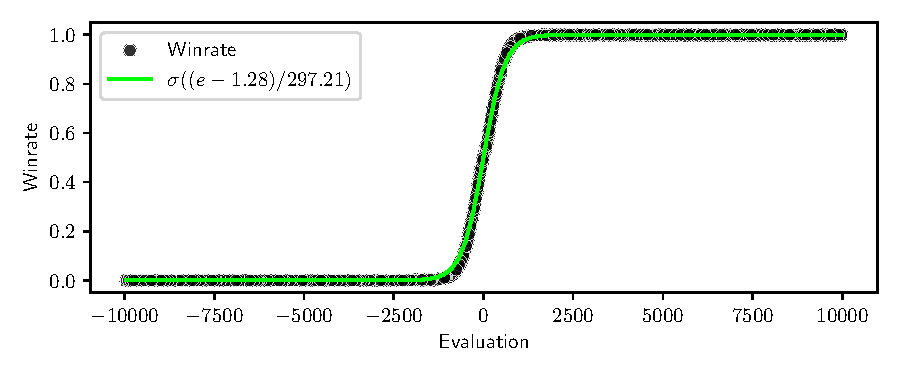
\includegraphics[width=\textwidth]{../assets/sigmoid_fit.pdf}}
\caption{WDL model function (sigmoid) fitted to 100 million evaluations in the dataset.}
\label{wdl-fit}
\end{figure}


During training, it is better to use a loss function with the target and output of the model in WDL-space instead of score-space. WDL-space has some advantages over score-space:

\begin{itemize}
\item Large evaluations are \enquote{closer} together in WDL-space., since having a score of 7500 or 8000 is not that different in terms of winrate (less than 1\%) than between 50 and 550 (more than 30\%). This is desirable because the evaluations don't need to be that precise when the outcome of the game is almost decided.
\item The result of a game can be interpolated in WDL-space. If we introduce a new parameter $\lambda$, we can interpolate the evaluation $f(p)$ and the game result $r$ (in WDL-space) using: $\lambda * \mathcal{W}(f(p)) + (1 - \lambda) * r$. This way, the information about the outcome of the game can be used to steer the network in the right direction. This is not implemented in this work.
\item Values in WDL-space are smaller than in score-space, so it avoids large gradients.
\end{itemize}




\subsubsection{Loss function}

The loss function chosen is mean squared error (MSE) with a power of 2.6 (the value used by the Stockfish's official trainer) given by

% q = (output / out_scaling).sigmoid()
% p = (target / in_scaling).sigmoid()
% loss = torch.pow(torch.abs(p - q), 2.6).mean()

\[
\mathcal{L}(y,f(x,\bm{W}))= \frac{1}{N} \sum_i^N \left| \mathcal{W}(y_i) - \mathcal{W}(f(x_i,\bm{W})) \right| ^{2.6}
\]

where\dots

\begin{enumerate}
\itemsep0em
\item $N$ is the number of samples.
\item $y$ are the target scores.
\item $f$ is the model.
\item $x$ are the inputs (encoded feature sets).
\item $\bm{W}$ are the parameters of the model.
\item $\mathcal{W}$ is the winrate function that maps from score-space to WDL-space.
\end{enumerate}

\subsection{Method 2: PQR triplets}

This is an additional technique I wanted to try, described in \cite{dlchess:2014}. The method is based in the assumption that moves in the training data are better than random. In the blog they used human moves from the Lichess database \cite{lichessdb}, so they rely in the fact that humans make good or near-optimal moves most of the time, even if they are amateurs. In my case I will use Stockfish moves, which are extremely good. This method does not use the scores provided, it will have to learn them from scratch. Of course this is way harder to train but I'm curious to see how far the following idea can go.

Remember that we are trying to obtain a function $f$ (the model) to give an evaluation of a position. The idea is based on the following two principles:

\begin{enumerate}
\item For two positions in succession $p \rightarrow q$ observed in a game, we will have $f(p)=-f(q)$. This comes from the fact that the game is zero-sum.
\item Going from the position $p$, not to observed position $q$, but to a \textit{random} position $p \rightarrow r$, we must have $f(r) > f(q)$ because the random move is better for the next player and worse for the player that made the move.
\end{enumerate}

If this reasonable assumptions hold, a loss function that expresses the equality in (1) and the inequality in (2) can be constructed.

% Consider an optimal $f$, that outputs $-1,0,1$ depending on who wins.
% With infinite compute, $f$ would be the result of running minimax to the end of the game, since minimax always finds optimal moves.

\subsubsection{Loss function}

The loss function is sum of the negative log-likelihood of the inequalities: ${f(r) > f(q)}$, ${f(p) > - f(q)}$ and ${f(p) < -f(q)}$. The last two are a way to express the equality $f(p)=-f(q)$. Each term is the negative log-likelihood function of the known Bradley-Terry model \cite{bradley-terry:1952}, that models the probability of an item (in our case a position) \enquote{beating} another item.

The loss function is given by

\begin{align*}
\mathcal{L}(x^p, x^q, x^r, \bm{W})=
\frac{1}{N}
\sum_i^N
& -\log\left(\sigma(\hat{r}_i - \hat{q}_i)\right) \\
& -\log\left(\sigma(\hat{p}_i + \hat{q}_i)\right) \\
& -\log\left(\sigma(-(\hat{p}_i + \hat{q}_i))\right)
\end{align*}

where\dots

\begin{enumerate}
\itemsep0em
\item $N$ is the number of samples.
\item $x^i$ are the inputs (encoded feature sets) for the $i \in \{p,q,r\}$ positions.
\item $f$ is the model.
\item $\bm{W}$ are the parameters of the model.
\item $
\hat{p}_i = \frac{f(x^p_i, \bm{W}) - a}{b},\text{ }
\hat{q}_i = \frac{f(x^q_i, \bm{W}) - a}{b},\text{ }
\hat{r}_i = \frac{f(x^r_i, \bm{W}) - a}{b}
$, where $a$ and $b$ are the parameters of the WDL model. Note that quantization is happening in this method too, so the output of the model must be scaled appropriately.
\end{enumerate}



Let's break down the loss function in a more intuitive way. We want the loss function to be small when the model is generating the correct evaluations and large when it is not. Let's look at the graph of the function $-\log(\sigma(x))$:

\begin{figure}[H]
\centering
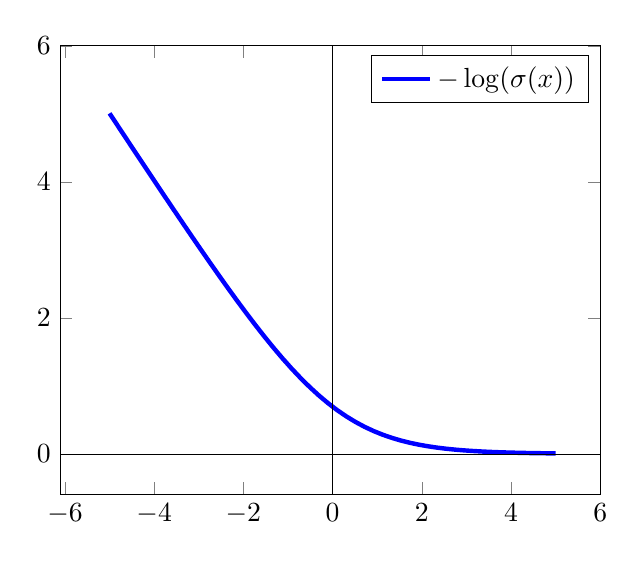
\begin{tikzpicture}
\begin{axis}[xmax=6,ymax=6, samples=50]
\addplot[blue, ultra thick] (x,{-ln(1/(1+e^-x))});
\draw[ultra thin] (axis cs:\pgfkeysvalueof{/pgfplots/xmin},0) -- (axis cs:\pgfkeysvalueof{/pgfplots/xmax},0);
\draw[ultra thin] (axis cs:0,\pgfkeysvalueof{/pgfplots/ymin}) -- (axis cs:0,\pgfkeysvalueof{/pgfplots/ymax});
\addlegendentry{$-\log(\sigma(x))$}
\end{axis}
\end{tikzpicture}
\end{figure}

The function approaches 0 when $x$ grows, and approaches $\infty$ when $x$ goes to $-\infty$.

Let's look at each of the terms:

\begin{enumerate}
\itemsep0em
\item $-\log(\sigma(\hat{r} - \hat{q}))$: This term is small when $\hat{r} > \hat{q}$, and large when $\hat{r} < \hat{q}$.
\item $-\log(\sigma(\hat{p} + \hat{q}))$: This term is small when $\hat{p} > -\hat{q}$, and large when $\hat{p} < -\hat{q}$.
\item $-\log(\sigma(-(\hat{p} + \hat{q}))$: This term is small when $\hat{p} < -\hat{q}$, and large when $\hat{p} > -\hat{q}$.
\end{enumerate}

The term (1) holds the inequality $f(r) > f(q)$, and the terms (2) and (3) hold the equality $f(p) = -f(q)$. The loss function is the sum of the three terms, so the model is encouraged when it satisfies the inequalities and penalized when it does not.

\subsection{Setup}


The project is written in two languages: Rust and Python. The Rust part is used to process dataset files, generate statistics and provide final training batches for Python to consume. The Python part defines the Pytorch model, runs the training loop, quantizes the model and runs the evaluations. \\

The training process is started by running a Python script (\texttt{scrips/train.py}) and it requires to define the model architecture (number of neurons on each layer), general training parameters (learning rate, batch size, epochs, checkpoints, etc) and the feature set to use, which in turn determines the size of the batches. For example, if PQR is used, the size of a sample is 3 times the size of the feature set times two (because it is siamese), and if it is score target, it is the size of the feature set times two plus 1 for the target score.

To orchestrate training runs, the platform Weights and Biases (WandB) is used. It provides automatic sweeping of hyperparameter, logging of metrics and visualizations. Results are exported from the platform in CSV and then processed by Python scripts. \\

The training data has to be converted to an actual tensor of floats to be consumed by Pytorch. This is done by a Rust subprocess running the subcommand \texttt{batch-loader} that read the training data file and generates training batches for the specified feature set in a shared memory buffer.

The batch generation process is heavily parallelized. Let's call $N$ the number of threads ($N=8$ was used). When the process starts, it splits the dataset file into $N$ equal parts and assigns each part to a thread. Each thread reads samples sequentially and builds the batch in a buffer. The buffer is then sent to the main thread where it is copied to the shared memory buffer.

The Python script copies the data from the shared buffer at the start of each iteration, allowing Rust to generate the next batch (in the CPU) while Pytorch is training the current batch (in the GPU). To coordinate the memory access between the two processes, a single byte is sent using standard I/O. The sequence of a training loop is shown in Figure \ref{training-loop}.

\begin{figure}[H]
\centering
\makebox[\textwidth]{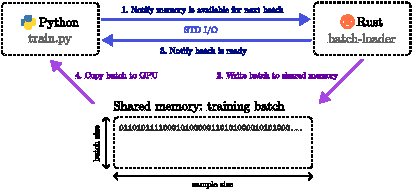
\includegraphics[width=\textwidth]{../assets/training-loop.pdf}}
\caption{Sequence of steps to send a batch from the \texttt{batch-loader} subprocess in Rust to Pytorch.}
\label{training-loop}
\end{figure}

Given that the input vector is multiple-hot encoded, the data written by the Rust process are not float values. Instead, they are 64-bit integers acting as a bitset. Before passing the vector to the model, it is expanded into floats. This means 64 floats can be packed into a single 64-bit integer, meaning a \textbf{96.875\%} reduction in memory usage (from 256 to 8 bytes). The speedup obtained by this optimization was substantial. The compression can be further improved using sparse tensors, but it is not implemented in this work. \\

%\begin{figure}[H]
%\centering
%\makebox[\textwidth]{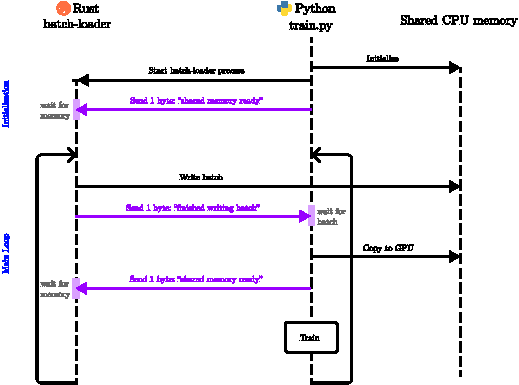
\includegraphics[width=\textwidth]{../%assets/training.pdf}}
%\caption{assad.}
%\end{figure}

% [evaluation?]
% [a esta seccion se le pueden agregar mil cosas]
% [multithreaded, perf]
% decir que en "All" tengo 450 it/s (7.3M pos/sec)

